\newpage
\section{Copernicus e Sentinel-2}
\subsection{Il programma spaziale Europeo Copernicus}
Copernicus \cite{COPERNICUS_INFO} è il nome dell’innovativo programma di 
monitoraggio del pianeta Terra portato avanti dall’Unione Europea.
Il programma è coordinato e gestito dalla Commissione europea ed è attuato in 
collaborazione con gli Stati membri, l'Agenzia spaziale europea (ESA), 
l'Organizzazione europea per l'esercizio dei satelliti meteorologici (EUMETSAT), 
il centro europeo per le previsioni meteorologiche a medio termine (CEPMMT), 
le agenzie dell'UE e il Mercator Océan.
Il programma Copernicus, iniziato nel 2014, si propone di fornire 
informazioni di libero accesso in merito alle condizioni del pianeta, 
al fine di informare e aiutare nelle decisioni le autorità, i cittadini, i 
ricercatori e le organizzazioni. Questo per offrire servizi in sei 
campi: atmosfera, ambiente marino, 
territorio, cambiamenti climatici, sicurezza ed emergenze. 
Il programma Copernicus è costituito da un insieme di satelliti in orbita 
e da altri sistemi aerei, terrestri o marittimi (detti in situ, ovvero non spaziali), 
i quali generano enormi quantità di dati su misurazioni e fotografie del pianeta.
Questi dati vengono poi resi disponibili al pubblico  
in seguito a elaborazioni e archiviazioni.

\subsection{Le missioni Sentinel}

I satelliti principali utilizzati dal programma sono quelli appartenenti 
alla classe \textit{Sentinel} (Sentinelle), i quali sono stati progettati e 
lanciati dall'Agenzia Spaziale Europea (ESA) appositamente per il programma 
Copernicus. Vengono utilizzati 
anche satelliti preesistenti o commerciali per dati complementari (in questo caso si parla 
di missioni partecipanti). Il programma ha attualmente attive 6 missioni Sentinel, ognuna delle 
quali è basata su una costellazione di 2 satelliti: questi ultimi viaggiano sulla stessa orbita 
però sfasati di 180° tra di loro, in modo da garantire tempi di rivisitazione 
(passaggio sopra lo stesso punto della Terra) ottimali. 
Questi satelliti trasportano sensori ottici, radar e strumenti di imaging 
dedicati al monitoraggio delle terre, degli oceani e dell’atmosfera.
I dati sentinel sono accessibili tramite il portale messo a disposizione dall'ESA: 
Sentinel Scientific Data Hub (https://scihub.copernicus.eu/) .

\subsubsection{Sentinel-1}
Sentinel-1 è una missione in orbita quasi-polare \cite{ORBITA_POLARE} (angolo di inclinazione rispetto 
l’equatore pari a 98°) iniziata nel 2014 è costituita dai satelliti Sentinel-1A e Sentinel-1B, 
aventi un sistema radar ad apertura sintetica (che invia e riceve impulsi lateralmente). Lo 
scopo è l’imaging radar della Terra diurno e notturno per il monitoraggio terrestre, 
marittimo e climatico.

% \begin{figure}[H]
%     \centering
%     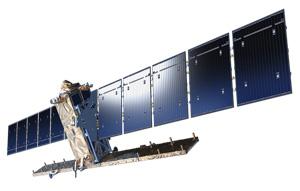
\includegraphics[width=0.3\textwidth]{Immagini/Satelliti/Sentinel_1.png}
%     \caption{Modello di sentinel-1}
% \end{figure}

\subsubsection{Sentinel-2}

Sentinel-2 è una missione in orbita quasi-polare eliosincrona \cite{ELIO_SINCRONA} 
(ovvero sincrona con il sole 
quindi garantisce sempre la stessa luminosità) iniziata nel 2015 è costituita dai satelliti 
Sentinel-2A (lanciato il 23 giugno 2015) e Sentinel-2B (lanciato il 7 marzo 2017). 
Entrambi i satelliti hanno una durata prevista di 7 anni, pertanto saranno 
successivamente sostituiti dai satelliti Sentinel-2C, lanciato il 5 settembre 2024, e 
dal Sentinel-2D.
L’obiettivo è fornire immagini ad alta risoluzione per il 
monitoraggio del territorio, dei cambiamenti climatici, e delle emergenze. 
La copertura garantita dalla missione comprende tutte le terre continentali, comprese
tra le latitudini $56°S$ e $84°N$, i mari fino a $20 km$ dalle coste, tutte le isole europee e
quelle extra-europee con superficie maggiore di $100 km^2$, il Mar Mediterraneo e tutti
i mari chiusi. 

\subsubsection{Sentinel-3}
Sentinel-3 è una missione iniziata nel 2016 costituita dai satelliti Sentinel-3A e Sentinel
3B: monitora la superficie del mare e misura le temperature marine e terrestri, fornendo 
dati ottici, radar e altimetrici. L’obiettivo è il monitoraggio climatico, ambientale e 
oceanografico.

% \begin{figure}[H]
%     \centering
%     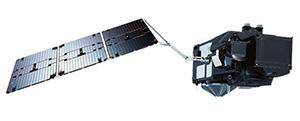
\includegraphics[width=0.3\textwidth]{Immagini/Satelliti/Sentinel_3.png}
%     \caption{Modello di sentinel-3}
% \end{figure}

\subsubsection{Sentinel-4}
Sentinel-4 è una missione non ancora operativa che fornirà dati sulla composizione 
atmosferica (concentrazioni di gas, aerosol e altre componenti).

% \begin{figure}[H]
%     \centering
%     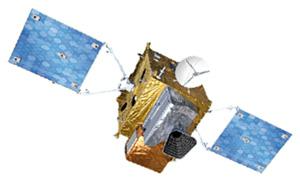
\includegraphics[width=0.3\textwidth]{Immagini/Satelliti/Sentinel_4.png}
%     \caption{Modello di sentinel-4}
% \end{figure}

\subsubsection{Sentinel-5}
Sentinel-5 è una missione non ancora operativa che monitorerà la composizione 
atmosferica: al momento è stato lanciato solo il satellite Sentinel-5P (Precursor) nel 2017, 
che sta rilevando provvisoriamente i dati sulla qualità dell’aria, sul clima e sulle 
radiazioni solari. 

% \begin{multicols}{2}
%     {
%         \begin{figure}[H]
%             \centering
%             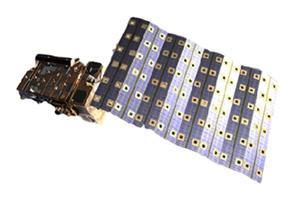
\includegraphics[width=0.25\textwidth]{Immagini/Satelliti/Sentinel_5.png}
%             \caption{Modello di sentinel-5}
%         \end{figure}
%     }
%     {
%         \begin{figure}[H]
%             \centering
%             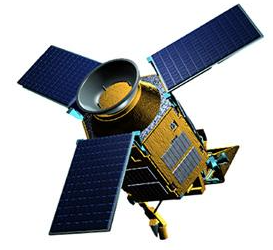
\includegraphics[width=0.25\textwidth]{Immagini/Satelliti/Sentinel_5P.png}
%             \caption{Modello di sentinel-5P}
%         \end{figure}
%     }
% \end{multicols}

\subsubsection{Sentinel-6}
Sentinel-6 è una missione non ancora operativa che misurerà il livello del mare per studi 
su clima e oceanografia. Al momento è stato lanciato solo uno dei satelliti.

% \begin{figure}[H]
%     \centering
%     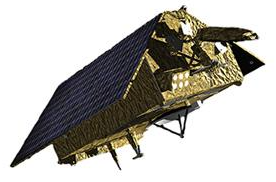
\includegraphics[width=0.3\textwidth]{Immagini/Satelliti/Sentinel_6.png}
%     \caption{Modello di sentinel-6}
% \end{figure}

\subsubsection{Satelliti attualmente in funzione}
I satelliti dedicati attualmente in orbita sono Sentinel-1A e Sentinel-1B, Sentinel-2A e 
Sentinel-2B, Sentinel-3A e Sentinel-3B, Sentinel-5P e Sentinel-6A 


\subsection{Caratteristiche di Sentinel-2}
I satelliti Sentinel-2 viaggiano ad una quota media di 786 km, hanno una swath (area 
analizzata dal satellite) che misura 290 km in larghezza e hanno un frequenza di 
rivisitazione complessiva è elevata (2-5 giorni) \cite{SENTINEL2_2,SENTINEL2_3, ALL_ABOUT_SENTINEL2}.

\begin{figure}[H]
    \centering
    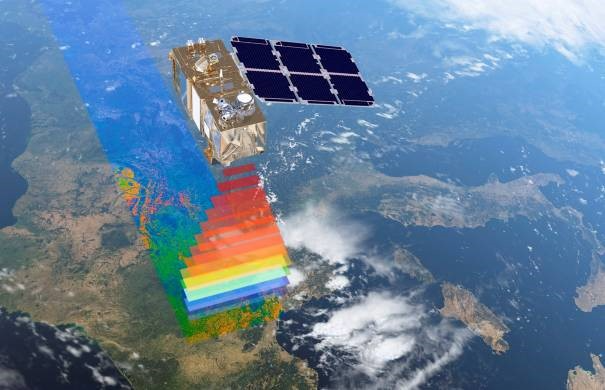
\includegraphics[width=0.5\textwidth]{Immagini/Satelliti/funzionamento_satellite.png}
    \caption{Rappresentazione di un satellite sentinel-2 \cite{immagini_multispettrali2}. }
\end{figure}

I satelliti Sentinel-2 si basano su un sistema di telerilevamento 
passivo, che non emette energia ma registra quella solare riflessa dagli 
oggetti presenti sulla superficie terrestre (a differenza del sistema radar, 
che è attivo quindi invia gli impulsi).

Le immagini prodotte sono multispettrali, perché la quantità di energia riflessa 
viene rilevata dal sensore attraverso diversi intervalli di lunghezze d’onda.
L'acquisizione delle informazioni avviene utilizzato un sistema 
\textit{push-broom}, nel quale due
fila di \textit{detector} (rilevatori), registrano i dati dello swath man mano che il 
satellite procede lungo l’orbita  \cite{ALL_ABOUT_SENTINEL2}. 

\begin{figure}[H]
    \centering
    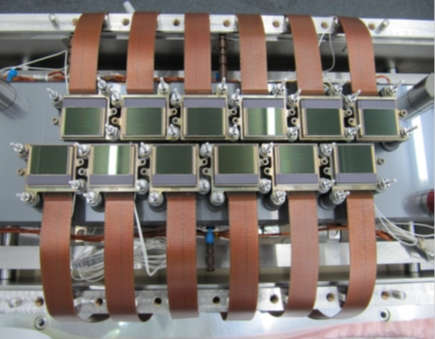
\includegraphics[width=0.3\textwidth]{Immagini/Satelliti/rilevatori_S2.png}
    \caption{Rappresentazione dei rilevatori \cite{ALL_ABOUT_SENTINEL2}.}
\end{figure}

Il rilevatore elettronico utilizzato è di tipo CCD (Charge coupled device) 
ed è costituito da una matrice di pixel, che in base alla quantità di energia 
ricevuta, assegna dei numeri (detti \textit{digital numbers}) ad ogni pixel. 
Questi \textit{digital numbers} (DN) rappresentano la radianza, 
misurata con una risoluzione radiometrica di 12 bit.

I \textit{digital numbers} misurati, vengono poi trasformati in toni di grigio 
per la visualizzazione: ad una maggiore radianza corrisponde un tono più chiaro 
(gli oggetti più chiari riflettono più energia, mentre quelli più scuri 
ne assorbono di più). 
Questo processo permette di generare immagini in bianco e nero per ogni banda spettrale.

La luce riflessa dalla Terra e dalla sua atmosfera verso lo 
MSI (MultiSpectral Instrument) viene raccolta da un telescopio a tre specchi (M1, M2 e M3) e 
focalizzata, tramite un divisore di fascio, su due \textit{Focal Plane Assemblies} (FPA): 
uno per le dieci lunghezze d'onda VNIR e uno per le tre lunghezze d'onda SWIR.
Successivamente i 12 rilevatori, presenti in ogni FPA, registrano la luce incidente, 
convertendola in dati digitali\cite{ALL_ABOUT_SENTINEL2}. 
%Dove ciascuno di questi FPA è composto da 12 rilevatori \cite{ALL_ABOUT_SENTINEL2}. 

\begin{figure}[H]
    \centering
    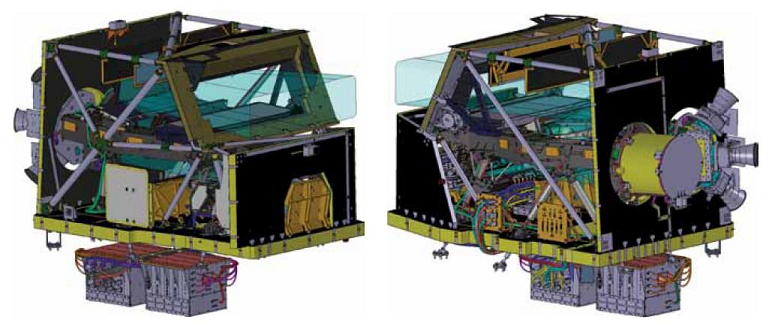
\includegraphics[width=0.5\textwidth]{Immagini/Satelliti/struttura_sentinel2_1.png}
\end{figure}

\begin{figure}[H]
    \centering
    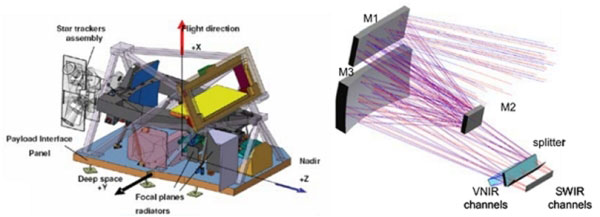
\includegraphics[width=0.7\textwidth]{Immagini/Satelliti/struttura_sentinel2_2.png}
    \caption{Rappresentazione dell'MSI \cite{ALL_ABOUT_SENTINEL2}.}
\end{figure}


Questo permette all'MSI del satellite di acquisire 4 bande nel visibile e 
vicino infrarosso con risoluzione spaziale $10m$, 6 bande nell'infrarosso 
con risoluzione spaziale $20m$ e 3 bande con risoluzione $60m$ di cui una nel 
blu e due nell'infrarosso \cite{MSI_SENTINEL2,ALL_ABOUT_SENTINEL2}.
Per risoluzione spaziale si intende a quale dimensione corrisponde un pixel 
nell'immagine telerilevata, ovvero la distanza coperta da un pixel \cite{ALL3_REMOTE_SENSING}.

\begin{figure}[H]
    \centering
    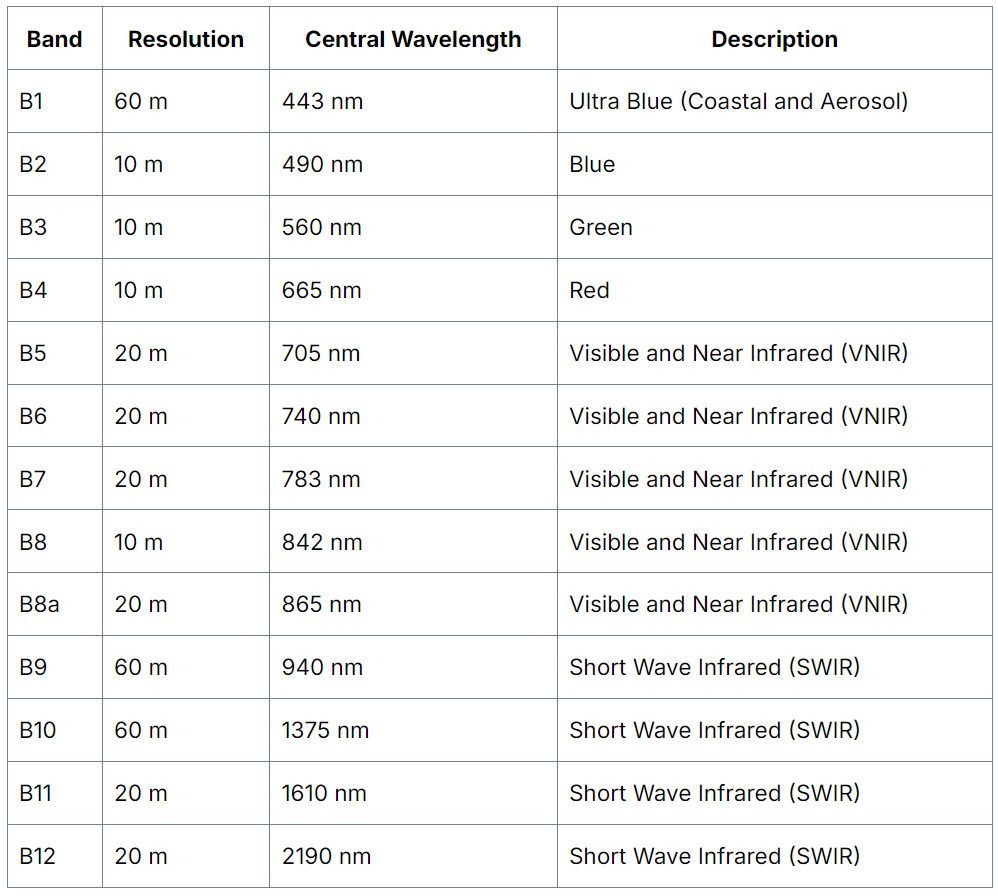
\includegraphics[width=0.70\textwidth]{Immagini/Generiche/Sentinel2_bands_table.png}
    \caption{Caratteristiche delle diverse bande \cite{Tabella_bande, COMBINAZIONE_BANDE_SENTINEL2} .}
    \label{fig:Tabella_bande_s2}
\end{figure}

\subsection{Combinazione delle bande di sentinel-2}
Le diverse bande, oltre a poter essere visualizzate singolarmente in scala di grigi, 
possono essere combinate per mettere in risalto diverse informazioni dell'immagine
\cite{COMBINAZIONE_BANDE_SENTINEL2, SENTINEL2_1_e_bands}.
Alcune delle molte combinazioni che possono essere ottenute utilizzando le bande di 
sentinel-2 sono:

\begin{itemize}
    \item \textbf{Natural Color (B4, B3, B2)}: utilizza i canali 
    rosso (B4), verde (B3) e blu (B2). Il suo scopo è visualizzare le immagini 
    con colori naturali così come la vedrebbero 
    naturalmente gli esseri umani.

    \begin{figure}[H]
        \centering
        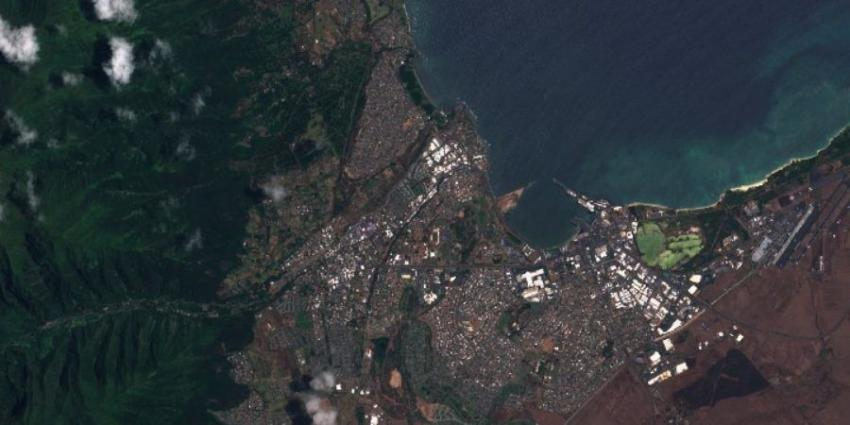
\includegraphics[width=0.6\textwidth]{Immagini/Satelliti/Sentinel-2-Natural-Color-850x425.jpg}
        \caption{Rappresentazione Natural Color.}
    \end{figure}

    \item \textbf{Color Infrared (B8, B4, B3)}: questa combinazione di bande è 
    pensata per enfatizzare la vegetazione sana e non sana. 
    La banda del vicino infrarosso (B8), è particolarmente efficace nel 
    riflettere la clorofilla. Per questo, in un'immagine infrarossa a colori, 
    la vegetazione più densa è rossa. Ma le aree urbane sono bianche.
    
    \begin{figure}[H]
        \centering
        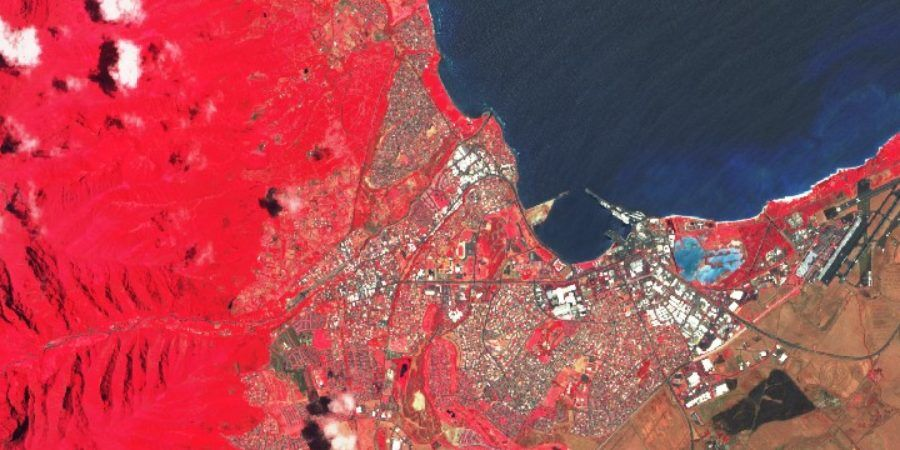
\includegraphics[width=0.6\textwidth]{Immagini/Satelliti/Sentinel-2-Color-Infrared.jpg}
        \caption{Rappresentazione Color Infrared.}
    \end{figure}
    
    \item \textbf{Short-Wave Infrared (B12, B8A, B4)}: utilizza le bande 
    SWIR (B12), NIR (B8A) e Rosso (B4). Questa composizione mostra la vegetazione in 
    varie tonalità di verde. In generale, le tonalità di verde più scure indicano una
    vegetazione più densa. Mentre il marrone può indicare un terreno privo di vegetazione 
    o un'area edificata.
    \begin{figure}[H]
        \centering
        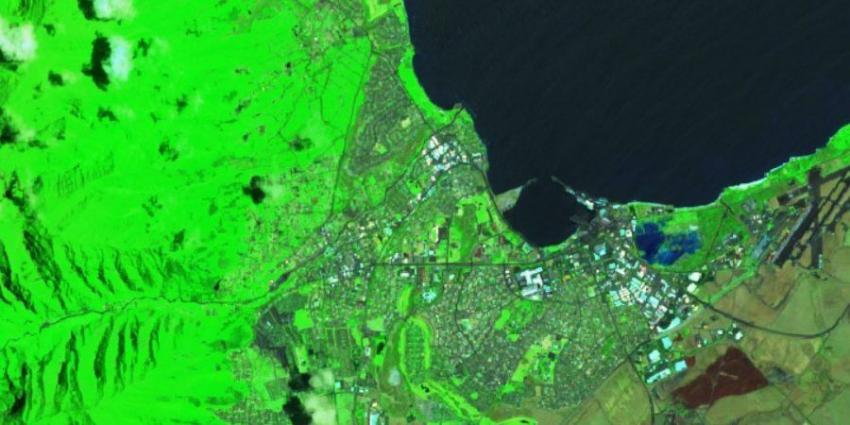
\includegraphics[width=0.6\textwidth]{Immagini/Satelliti/Sentinel-2-Shortwave-Infrared-850x425.jpg}
        \caption{Rappresentazione Short-Wave Infrared.}
    \end{figure}
    
    \newpage
    \item \textbf{Vegetation Index (B8-B4)/(B8+B4)}: Poiché che la 
    vegetazione ha una forte capacità di riflettere la radiazione 
    nel vicino infrarosso (Near Infrared, NIR) e di assorbire quella 
    nella banda del rosso, l'indice di vegetazione è utile per 
    quantificare la quantità di vegetazione presente in un'area. 
    
    \begin{figure}[H]
        \centering
        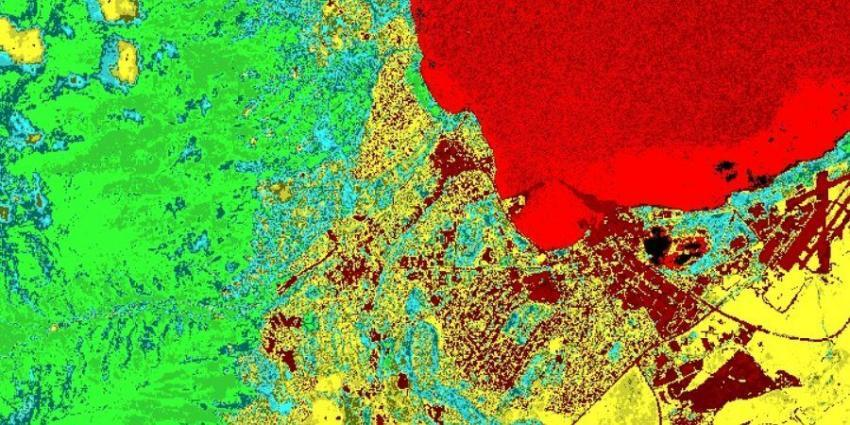
\includegraphics[width=0.6\textwidth]{Immagini/Satelliti/Sentinel-2-Vegetation-Index-850x425.jpg}
        \caption{Rappresentazione Vegetation Index.}
    \end{figure}
    
    \item \textbf{Moisture Index (B8A-B11)/(B8A+B11)}: è ideale per individuare lo 
    stress idrico nelle piante. Utilizza le onde corte e il vicino infrarosso per 
    generare un indice del contenuto di umidità. In generale, la vegetazione più 
    umida ha valori più alti. Ma valori di indice di umidità più bassi suggeriscono 
    che le piante sono sotto stress a causa di umidità insufficiente.
    
    \begin{figure}[H]
        \centering
        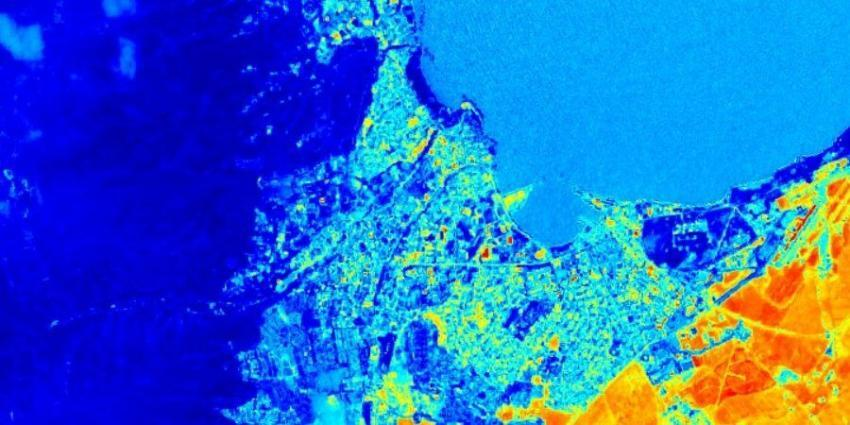
\includegraphics[width=0.6\textwidth]{Immagini/Satelliti/Sentinel-2-Moisture-Index-850x425.jpg}
        \caption{Rappresentazione Moisture Index.}
    \end{figure}

\end{itemize}
